\documentclass[11pt,a4paper]{article}
\usepackage[utf8]{inputenc}
\usepackage[T1]{fontenc}
\usepackage[margin=1in]{geometry}
\usepackage{graphicx}
\usepackage{hyperref}
\usepackage{xcolor}
\usepackage{float}
\usepackage{listings}
\usepackage{upquote}
\usepackage{amsmath}

% Code listing style
\lstset{
    basicstyle=\ttfamily\small,
    breaklines=true,
    breakatwhitespace=false,
    frame=single,
    numbers=left,
    numberstyle=\tiny,
    backgroundcolor=\color{gray!10},
    keywordstyle=\color{blue},
    commentstyle=\color{green!50!black},
    stringstyle=\color{red},
    showstringspaces=false
}

\title{\textbf{Practice 2 - Stretch Robot Kinematics}}
\author{
    Robotics and Cyber-Physical Systems \\
    School of Sciences and Engineering \\
    Tecnol\'ogico de Monterrey
}
\date{}

\begin{document}

\maketitle

\section*{Introduction}

This practice introduces the fundamental concepts of robot control through six progressive parts. You will learn how to command joint velocities, read sensor state, implement position control, process input devices, layer commands with proportional blending, and integrate full teleoperation with autonomous behaviors.

Each part builds on the previous one, developing a complete understanding of how to control the Stretch robot through the \texttt{stretch\_toolkit} interface.

\subsection*{Before You Begin}

If you previously cloned this repository, update it to the latest version to ensure you have all the necessary files and recent improvements. \textbf{Important:} The update command below will overwrite any local changes you've made. If you have files you want to keep (such as solutions to previous activities), make a backup copy outside the repository folder before proceeding.

To update your repository:

\begin{lstlisting}[language=bash]
git pull
git fetch origin
git reset --hard origin/main
\end{lstlisting}

If dependencies were updated, synchronize your environment:

\begin{lstlisting}[language=bash]
uv sync
\end{lstlisting}

\section{Part 1: Joint Velocity Control}

The primary way to move the robot is through \texttt{controller.set\_velocities()}, which accepts a dictionary mapping joint names to normalized velocities in the range $[-1.0,\ 1.0]$:

\begin{lstlisting}[language=Python]
controller.set_velocities({
    "lift_up": 0.5,               # lift at 50% speed upward
    "arm_out": -1.0,              # arm retracting at full speed
    "head_pan_counterclockwise": 0.3,
})
\end{lstlisting}

Joint names follow a directional convention: positive values move in the named direction, negative values move in the opposite direction. Below is the full set of controllable joints:

\begin{center}
\begin{tabular}{|l|l|}
\hline
\textbf{Joint name} & \textbf{Positive direction} \\
\hline
\texttt{base\_forward} & Translate forward \\
\texttt{base\_counterclockwise} & Rotate left \\
\texttt{lift\_up} & Lift upward \\
\texttt{arm\_out} & Arm extend \\
\texttt{gripper\_open} & Open gripper \\
\texttt{wrist\_yaw\_counterclockwise} & Wrist yaw left \\
\texttt{wrist\_pitch\_up} & Wrist pitch up \\
\texttt{wrist\_roll\_counterclockwise} & Wrist roll left \\
\texttt{head\_pan\_counterclockwise} & Head pan left \\
\texttt{head\_tilt\_up} & Head tilt up \\
\hline
\end{tabular}
\end{center}

\subsection*{Activity}

Starting from \texttt{stretch\_boilerplate.py}, make the robot's head pan joint oscillate back and forth using a sine wave. The velocity sent to the joint at each tick should be:

\[
v(t) = \sin(\omega \cdot t), \quad \omega = 2.0
\]

where $t$ is the elapsed time in seconds and $\omega$ controls the oscillation speed.

\textbf{Steps:}
\begin{enumerate}
    \item Copy \texttt{stretch\_boilerplate.py} and rename it \texttt{p2\_1\_velocity.py}.
    \item Add \texttt{import math} at the top.
    \item Inside the loop, compute the velocity as $v(t) = \sin(\omega \cdot t)$ with $\omega = 2.0$, where \texttt{t} is already provided by the boilerplate as \texttt{controller.get\_time()}.
    \item Pass it to \texttt{controller.set\_velocities()} for the \texttt{head\_pan\_counterclockwise} joint.
    \item Run with \texttt{uv run p2\_1\_velocity.py} and observe the head panning.
    \item Experiment with different values of $\omega$ and observe the effect on oscillation speed.
\end{enumerate}

\textbf{Expected result:} The robot's head pans smoothly left and right in a continuous sinusoidal motion.

\begin{figure}[H]
    \centering
    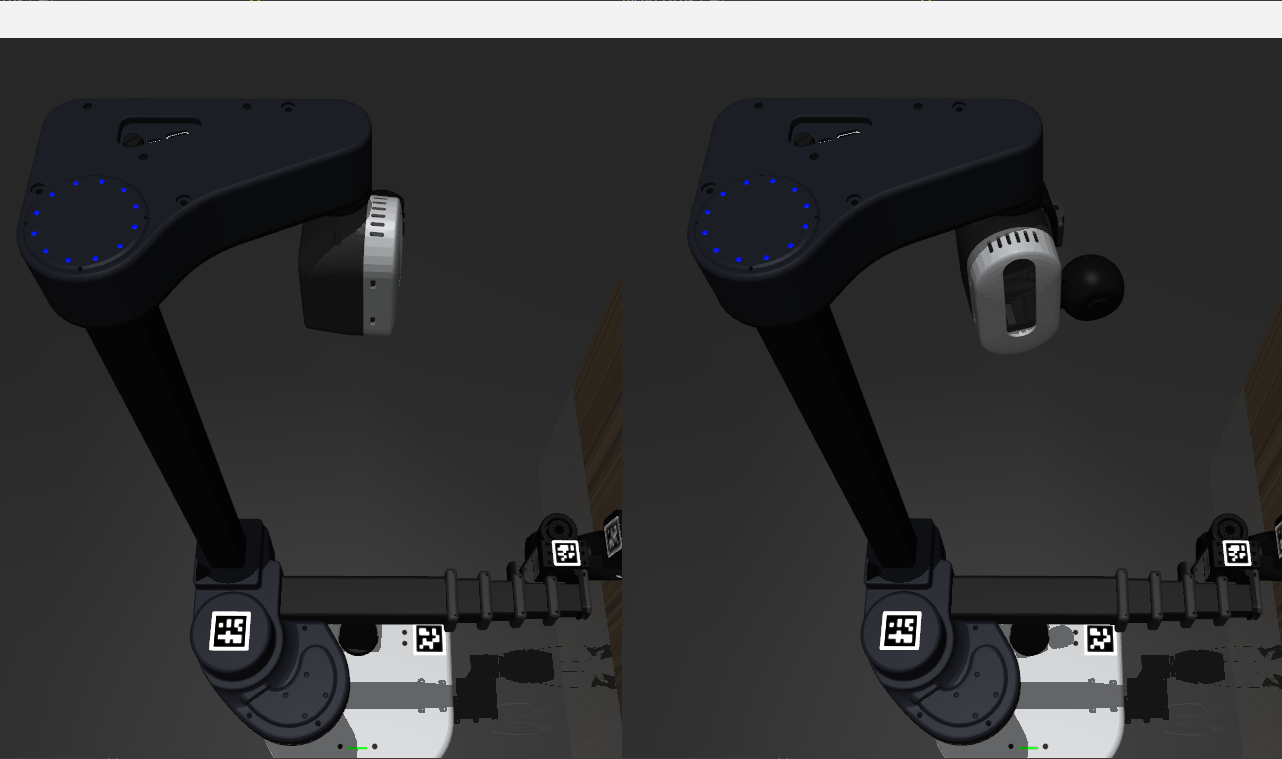
\includegraphics[width=0.6\textwidth]{head_pan.png}
    \caption{Robot head panning back and forth using sinusoidal velocity control.}
    \label{fig:head_pan}
\end{figure}

\section{Part 2: Reading Joint State}

In addition to sending commands, you can read the current position of every joint using \texttt{controller.get\_state()}, which returns a dictionary of joint positions:

\begin{lstlisting}[language=Python]
state = controller.get_state()
print(state["head_pan_counterclockwise"])  # current angle in radians
\end{lstlisting}

The keys match the joint names from Part 1. Linear joints (\texttt{lift\_up}, \texttt{arm\_out}) are in meters; all rotational joints are in radians. The base keys are odometry estimates and do not follow the directional naming convention:

\begin{center}
\begin{tabular}{|l|l|l|}
\hline
\textbf{Key} & \textbf{Unit} & \textbf{Description} \\
\hline
\texttt{base\_x} & meters & Base position along X axis (odometry) \\
\texttt{base\_y} & meters & Base position along Y axis (odometry) \\
\texttt{base\_theta} & radians & Base heading (odometry) \\
\hline
\texttt{lift\_up} & meters & Lift height \\
\texttt{arm\_out} & meters & Arm extension \\
\hline
\texttt{wrist\_yaw\_counterclockwise} & radians & Wrist yaw angle \\
\texttt{wrist\_pitch\_up} & radians & Wrist pitch angle \\
\texttt{wrist\_roll\_counterclockwise} & radians & Wrist roll angle \\
\texttt{head\_pan\_counterclockwise} & radians & Head pan angle \\
\texttt{head\_tilt\_up} & radians & Head tilt angle \\
\texttt{gripper\_open} & radians & Gripper opening angle \\
\hline
\end{tabular}
\end{center}

\subsection*{Activity}

Starting from your completed \texttt{p2\_1\_velocity.py}, add a live printout of the head pan joint position.

\textbf{Steps:}
\begin{enumerate}
    \item Copy \texttt{p2\_1\_velocity.py} and rename it \texttt{p2\_2\_state.py}.
    \item Inside the loop (after setting velocities), call \texttt{controller.get\_state()} and store the result.
    \item Print the value of the \texttt{head\_pan\_counterclockwise} key on each tick.
    \item Run with \texttt{uv run p2\_2\_state.py} and observe the printed values change as the head pans.
\end{enumerate}

\textbf{Expected result:} The terminal prints a stream of angle values (in radians) that oscillate as the head pans left and right.

\begin{lstlisting}
-2.7064544902869696
-2.7912609565602504
-2.8279074389854637
-2.8050669215428670
-2.7038859728338150
-2.6026917811471906
-2.4689193011507530
...
\end{lstlisting}

\section{Part 3: Position Control}

Sending raw velocities works well for continuous motion, but reaching a \emph{specific} position requires knowing when to stop. \texttt{StateController} handles this: given a desired joint position, it computes the velocity needed to move toward it each tick, and reports when the target has been reached.

Crucially, \texttt{StateController} does not bypass the velocity interface — it simply \emph{generates} the velocity commands for you. The robot is still driven through \texttt{controller.set\_velocities()}, keeping a single point of control over all motion.

\texttt{StateController} uses the same joint names as \texttt{set\_velocities()} and \texttt{get\_state()}.

Basic usage pattern:

\begin{lstlisting}[language=Python]
from stretch_toolkit import StateController

sc = StateController(controller, {"arm_out": 0.3})  # target: extend arm to 0.3 m

while True:
    controller.set_velocities(sc.get_command())   # drive toward target
    if sc.is_at_goal():
        break                                      # stop when reached
\end{lstlisting}

Optionally, you can track how far along a movement the robot is by calling \texttt{get\_progress(previous\_state)}, passing the state captured \emph{before} the movement began. It returns a dictionary mapping each joint to a value between 0.0 (not started) and 1.0 (arrived). This is not required for the activity, but can be useful for certain applications.

\begin{lstlisting}[language=Python]
initial = sc.get_current_state()

while not sc.is_at_goal():
    controller.set_velocities(sc.get_command())
    progress = sc.get_progress(initial)
    print(f"arm progress: {progress['arm_out']:.2f}")
\end{lstlisting}

\subsection*{Activity}

Make the arm joint bounce continuously between $0.1\,\text{m}$ and $0.3\,\text{m}$.

\textbf{Steps:}
\begin{enumerate}
    \item Copy \texttt{stretch\_boilerplate.py} and rename it \texttt{p2\_3\_position.py}.
    \item Import \texttt{StateController} from \texttt{stretch\_toolkit}.
    \item Before the loop, create a variable \texttt{target = 0.1} and create a \texttt{StateController} with \texttt{\{"arm\_out": target\}}.
    \item Inside the loop, call \texttt{sc.get\_command()} and pass the result to \texttt{controller.set\_velocities()}.
    \item When \texttt{sc.is\_at\_goal()} is \texttt{True}, use an if/else statement to toggle \texttt{target}: if it equals $0.1$, set it to $0.3$; otherwise set it to $0.1$. Then create a new \texttt{StateController} with the updated target.
    \item Run with \texttt{uv run p2\_3\_position.py} and watch the arm extend and retract.
\end{enumerate}

\textbf{Template for the toggle logic:}
\begin{lstlisting}[language=Python]
if sc.is_at_goal():
    if target == 0.1:
        target = 0.3
    else:
        target = 0.1
    sc = StateController(controller, {"arm_out": target})
\end{lstlisting}

\textbf{Expected result:} The arm smoothly travels from $0.1\,\text{m}$ to $0.3\,\text{m}$ and back, repeating indefinitely.

\textbf{Important:} Make sure this file works correctly before moving on. Parts 5 and 6 will build directly on this code, so it's essential that you have a working \texttt{p2\_3\_position.py} that bounces the arm reliably. Test it for at least a few complete cycles to verify the behavior.

\begin{figure}[H]
    \centering
    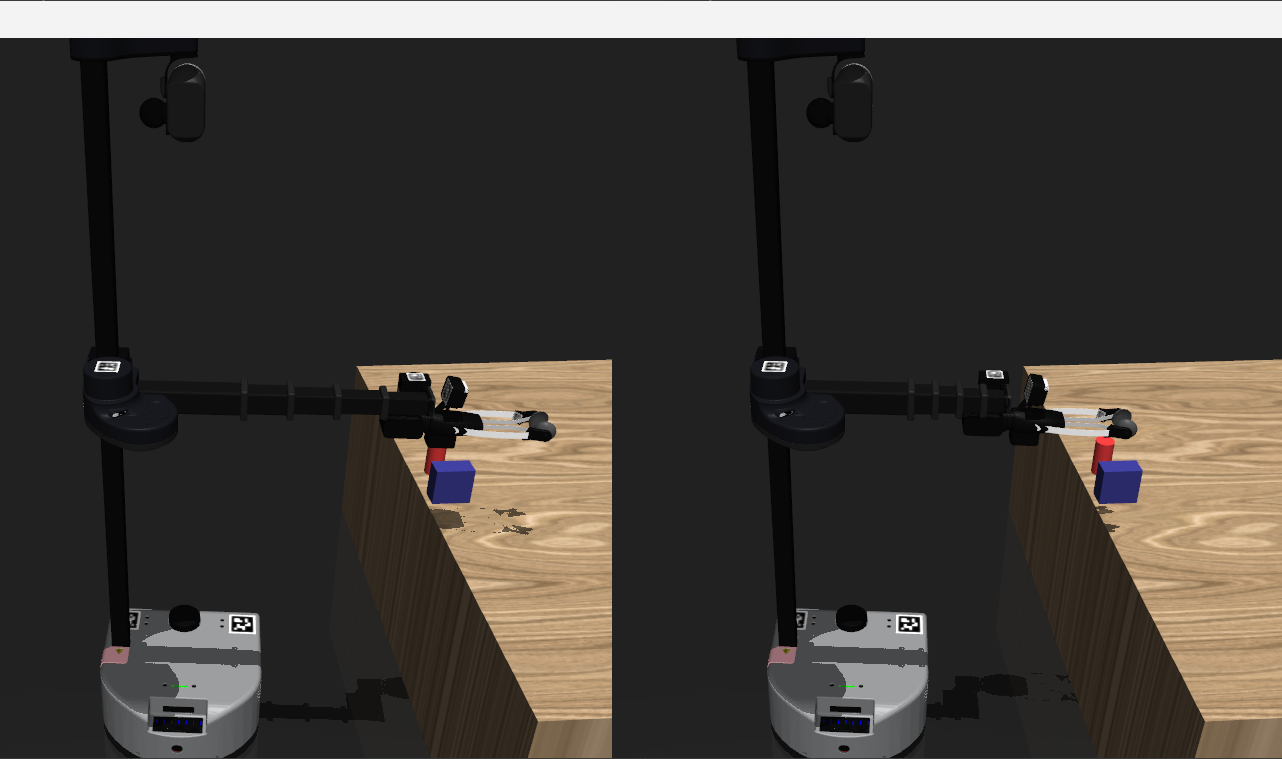
\includegraphics[width=0.6\textwidth]{arm_out.png}
    \caption{Robot arm extending and retracting using position control.}
    \label{fig:arm_out}
\end{figure}

\section{Part 4: Gamepad and Keyboard Input}

The \texttt{stretch\_toolkit.input} module provides a unified interface for reading gamepad buttons, analog axes, and keyboard keys. Import it with:

\begin{lstlisting}[language=Python]
import stretch_toolkit.input as inp
\end{lstlisting}

\subsection*{Buttons and keys: \texttt{is\_pressed}}

\texttt{inp.is\_pressed(name)} returns \texttt{True} as long as the given button or key is held down. It checks the gamepad first, then falls back to the keyboard.

\begin{lstlisting}[language=Python]
if inp.is_pressed("A"):          # gamepad A button
    ...
if inp.is_pressed("w"):          # keyboard 'w' key
    ...
\end{lstlisting}

The full set of gamepad button names is:

\begin{center}
\begin{tabular}{|l|l|}
\hline
\textbf{Name} & \textbf{Button} \\
\hline
\texttt{A}, \texttt{B}, \texttt{X}, \texttt{Y} & Face buttons \\
\texttt{LB}, \texttt{RB} & Bumpers \\
\texttt{LT}, \texttt{RT} & Triggers (also available as axes) \\
\texttt{L3}, \texttt{R3} & Stick clicks \\
\texttt{DPAD\_UP}, \texttt{DPAD\_DOWN}, \texttt{DPAD\_LEFT}, \texttt{DPAD\_RIGHT} & D-pad \\
\texttt{START}, \texttt{SLCT}, \texttt{GUIDE} & Menu buttons \\
\hline
\end{tabular}
\end{center}

\subsection*{Analog axes: \texttt{get\_axis}}

\texttt{inp.get\_axis(name)} returns a normalized float. Sticks return $[-1.0,\ 1.0]$; triggers return $[0.0,\ 1.0]$.

\begin{lstlisting}[language=Python]
lx = inp.get_axis("LX")   # left stick horizontal
rt = inp.get_axis("RT")   # right trigger (0.0 to 1.0)
\end{lstlisting}

Available axes:

\begin{center}
\begin{tabular}{|l|l|l|}
\hline
\textbf{Name} & \textbf{Source} & \textbf{Range} \\
\hline
\texttt{LX}, \texttt{LY} & Left stick & $[-1.0,\ 1.0]$ \\
\texttt{RX}, \texttt{RY} & Right stick & $[-1.0,\ 1.0]$ \\
\texttt{LT}, \texttt{RT} & Triggers & $[0.0,\ 1.0]$ \\
\texttt{DPAD\_X}, \texttt{DPAD\_Y} & D-pad & $\{-1,\ 0,\ 1\}$ \\
\hline
\end{tabular}
\end{center}

\subsection*{Single-frame detection: \texttt{rising\_edge}}

\texttt{inp.rising\_edge(name)} returns \texttt{True} exactly once — on the first frame a button goes down. Subsequent calls return \texttt{False} until the button is released and pressed again. This is useful for toggling state or triggering a one-shot action:

\begin{lstlisting}[language=Python]
if inp.rising_edge("A"):
    print("A was just pressed")   # fires once per press
\end{lstlisting}

\section{Part 5: Command Layering}

In practice, you often want to run an autonomous behavior while still being able to override it manually. The challenge is combining two command dictionaries — one from a controller or algorithm, one from the gamepad — without simply discarding one of them.

\texttt{merge\_proportional} solves this. It takes a \emph{primary} command (typically teleop) and a \emph{secondary} command (typically autonomous), and blends them based on how much the primary input is active:

\begin{lstlisting}[language=Python]
from stretch_toolkit import merge_proportional

merged = merge_proportional(cmd_primary, cmd_secondary)
controller.set_velocities(merged)
\end{lstlisting}

The blending rule per joint is:

\begin{itemize}
    \item If the primary input magnitude is below a deadband (default $0.05$), the secondary command is used unchanged.
    \item Otherwise, the primary input strength (0 to 1) determines how much the secondary is overridden: at full deflection the joint moves at full speed in the primary direction; at partial deflection the output is a weighted blend.
\end{itemize}

This means a light touch on the stick nudges the robot away from its autonomous target, while a full push takes over completely. Releasing the stick hands control back to the secondary command seamlessly.

A typical pattern combining autonomous position control with manual override looks like:

\begin{lstlisting}[language=Python]
from stretch_toolkit import controller, StateController, merge_proportional
import stretch_toolkit.input as inp

sc = StateController(controller, {"arm_out": 0.3})

while True:
    cmd_auto   = sc.get_command()
    cmd_teleop = {"arm_out": inp.get_axis("RX")}
    controller.set_velocities(merge_proportional(cmd_teleop, cmd_auto))
\end{lstlisting}

Here, moving the right stick overrides the autonomous arm motion proportionally; leaving the stick centered lets the \texttt{StateController} drive undisturbed.

\subsection*{Activity}

Starting from your completed \texttt{p2\_3\_position.py}, add a manual override that extends the arm fully while the \texttt{'v'} key is held.

\textbf{Steps:}
\begin{enumerate}
    \item Copy \texttt{p2\_3\_position.py} and rename it \texttt{p2\_5\_layering.py}.
    \item Inside the loop, build a primary command dict: set \texttt{"arm\_out"} to \texttt{1.0} if \texttt{inp.is\_pressed("v")} is \texttt{True}, otherwise \texttt{0.0}.
    \item Use \texttt{merge\_proportional} to merge the primary command with \texttt{sc.get\_command()}, and pass the result to \texttt{controller.set\_velocities()}.
    \item Run with \texttt{uv run p2\_5\_layering.py}. The arm should bounce as before. While holding \texttt{'v'}, it should override and extend fully.
\end{enumerate}

\textbf{Expected result:} The arm bounces between $0.1\,\text{m}$ and $0.3\,\text{m}$ autonomously, but pressing \texttt{'v'} overrides the motion and drives the arm toward full extension.

\begin{figure}[H]
    \centering
    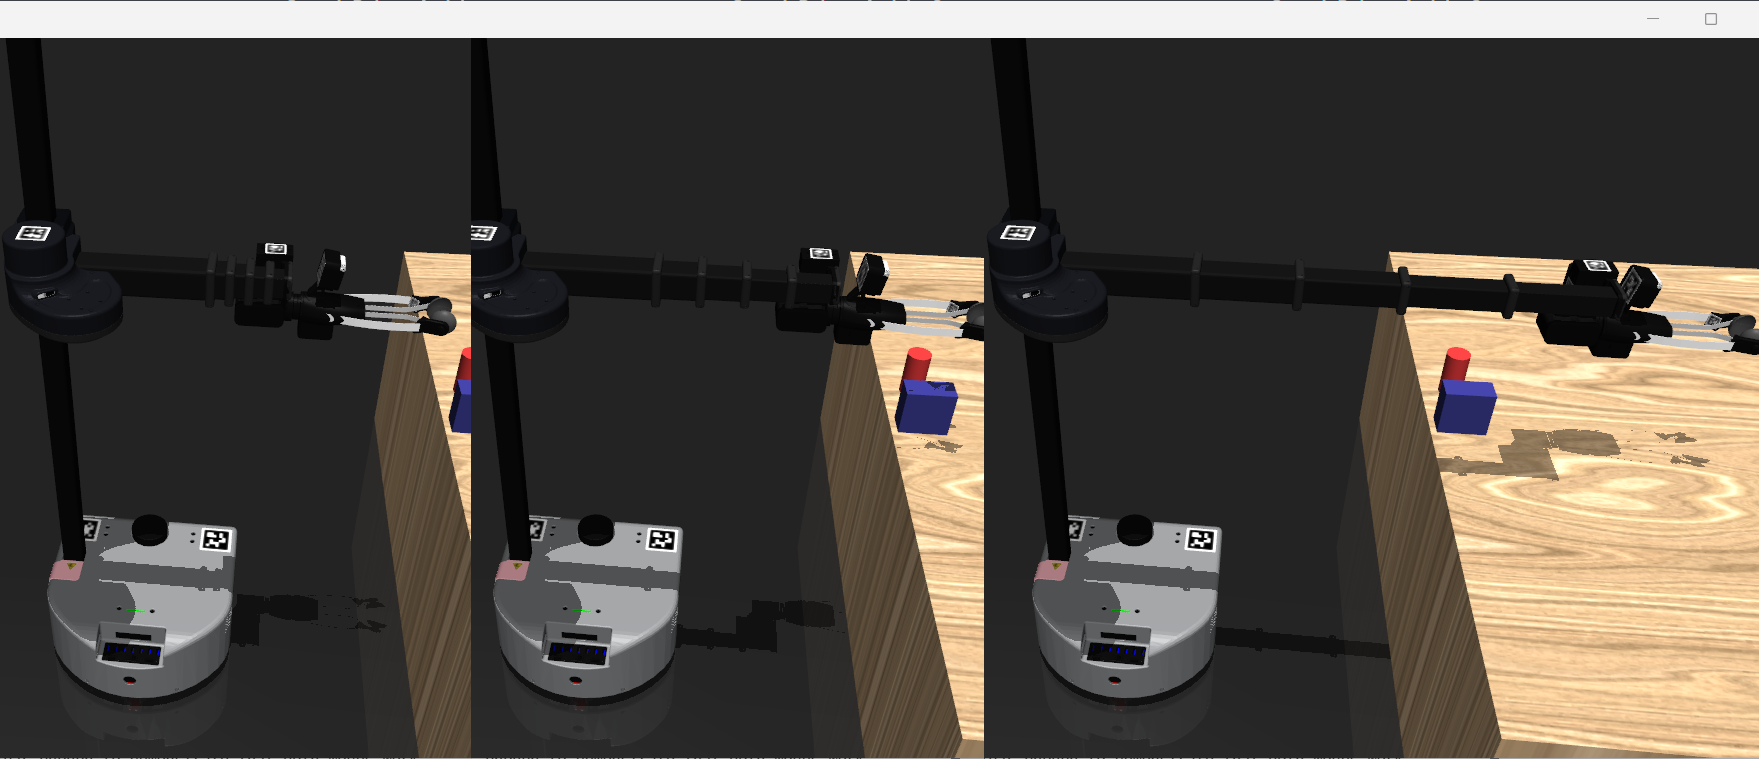
\includegraphics[width=0.6\textwidth]{arm_out_override.png}
    \caption{Manual override taking priority over autonomous position control.}
    \label{fig:arm_out_override}
\end{figure}

\section{Part 6: Full Teleop Override}

In Part 5, you built a manual override by constructing a primary command dict by hand. In practice, you want the operator to be able to override \emph{any} joint at any time using the full gamepad and keyboard mapping — not just a single hard-coded key.

\texttt{TeleopProvider} already knows how to read all joints from the input devices. Its \texttt{get\_manual\_override(cmd\_autonomous)} method combines this with \texttt{merge\_proportional} in a single call: it reads the current teleop input, uses it as the primary command, and blends it with the autonomous command you provide.

\begin{lstlisting}[language=Python]
from stretch_toolkit import controller, teleop, StateController

sc = StateController(controller, {"arm_out": 0.3})

while True:
    controller.set_velocities(teleop.get_manual_override(sc.get_command()))
\end{lstlisting}

This replaces both \texttt{teleop.get\_normalized\_velocities()} and the manual \texttt{merge\_proportional} call with a single line, while giving the operator proportional control over every joint simultaneously.

Additionally, pressing the \texttt{Y} key (or \texttt{y}) toggles between two modes:
\begin{itemize}
    \item \textbf{AUTONOMOUS mode} (default): Proportional blending — the operator can override any joint, but the autonomous command runs when inputs are idle.
    \item \textbf{MANUAL mode}: Pure teleop control — the autonomous command is ignored completely, and only the operator's inputs drive the robot.
\end{itemize}

\subsection*{Activity}

Starting from your completed \texttt{p2\_3\_position.py}, replace the raw \texttt{set\_velocities} call with a full teleop override.

\textbf{Steps:}
\begin{enumerate}
    \item Copy \texttt{p2\_3\_position.py} and rename it \texttt{p2\_6\_teleop\_override.py}.
    \item Import \texttt{teleop} from \texttt{stretch\_toolkit}.
    \item Replace \texttt{controller.set\_velocities(sc.get\_command())} with \texttt{controller.set\_velocities(teleop.get\_manual\_override(sc.get\_command()))}.
    \item Run with \texttt{uv run p2\_6\_teleop\_override.py}. The arm bounces as before, but now any mapped key or gamepad input can override any joint proportionally.
    \item Press \texttt{Y} (or \texttt{y}) to toggle to MANUAL mode. The arm stops bouncing and responds only to your inputs. Press \texttt{Y} again to return to AUTONOMOUS mode.
\end{enumerate}

\textbf{Expected result:} In AUTONOMOUS mode, the arm bounces while you can proportionally override any joint. In MANUAL mode, the arm stops bouncing and responds only to your direct teleop control. The toggle gives you instant control over whether autonomous behavior runs or not.

\section*{Deliverable}

Submit a video demonstrating your completed \texttt{p2\_6\_teleop\_override.py} program. The video should show:

\begin{enumerate}
    \item The robot arm bouncing autonomously between $0.1\,\text{m}$ and $0.3\,\text{m}$ in AUTONOMOUS mode.
    \item You using gamepad or keyboard inputs to proportionally override the arm's motion while it continues bouncing.
    \item You pressing the \texttt{Y} key to toggle to MANUAL mode (the arm should stop bouncing and respond only to your inputs).
    \item You controlling the robot manually in MANUAL mode.
    \item You pressing \texttt{Y} again to return to AUTONOMOUS mode (the arm should resume bouncing).
\end{enumerate}

The video should be clear enough to demonstrate that both modes work correctly and that the proportional override functions as expected. Keep the video concise — 30 to 60 seconds is sufficient.

\end{document}
